

\section{Nutrient and Fertilizers}

\subsection{Nutrient}

The analysis of soil properties based on Soil and Fertilizer data revealed that the majority of soil samples exhibited neutral pH levels (79.2\%). Additionally, organic matter content was predominantly medium to high, with 83.3\% falling within the medium range and 12.5\% classified as high. Nitrogen levels varied, with a significant proportion (45.8\%) in the medium range, conducive to healthy plant growth. Phosphorus levels were notably high, with 50\% of samples classified as high and the remaining 50\% as very high, suggesting adequate phosphorus availability for plant nutrition. Potash levels also demonstrated a diverse distribution, with the majority falling within the medium to high range. These results enhance our understanding of soil quality by highlighting subtle differences in important agricultural metrics that can guide targeted actions for optimal crop management (Table \ref{tab:soil_properties}).

\begin{table}[H]
    \centering
    \caption{Soil Properties and Their Interpretation}
    \label{tab:soil_properties}
    \begin{tabular}{llcc}
        \toprule
        \textbf{Variables} & \textbf{Scale} & \textbf{Interpretation} & \textbf{Percent (\%)} \\
        \midrule
        \textbf{pH} & 1--6.5 & Acidic & 20.8 \\
        & 6.5--7.5 & Neutral & 79.2 \\
        & 7.5--14 & Basic & 0 \\
        \midrule
        \textbf{Organic Matter} & $<$0.1 & Very Low & 0 \\
        & 1.1--2.5 & Low & 4.2 \\
        & 2.6--5 & Medium & 83.3 \\
        & 5.1--10 & High & 12.5 \\
        & $>$11 & Very High & 0 \\
        \midrule
        \textbf{Nitrogen} & $<$0.05 & Very Low & 0 \\
        & 0.051--0.10 & Low & 4.2 \\
        & 0.11--0.20 & Medium & 45.8 \\
        & 0.21--0.4 & High & 50 \\
        & $>$0.41 & Very High & 0 \\
        \midrule
        \textbf{Phosphorus} & $<$10 & Very Low & 0 \\
        & 11--30 & Low & 0 \\
        & 31--55 & Medium & 0 \\
        & 56--110 & High & 50 \\
        & $>$110 & Very High & 50 \\
        \midrule
        \textbf{Potash} & 0--55 & Very Low & 0 \\
        & 56--110 & Low & 0 \\
        & 111--280 & Medium & 41.7 \\
        & 281--500 & High & 54.2 \\
        & $>$501 & Very High & 4.2 \\
        \bottomrule
    \end{tabular}
\end{table}

Descriptive statistics of soil nutrients (pH, Organic Matter, Nitrogen, Phosphorus, and Potash) are presented in Table \ref{tab:descriptive_statistics}, showing the Minimum, Maximum, Mean, and Standard Deviation of each nutrient. This table complements the findings of Table \ref{tab:soil_properties} by providing measures of central tendency and variability for each soil nutrient.

\begin{table}[H]
    \centering
    \caption{Descriptive statistics of soil nutrients and total yield}
    \label{tab:descriptive_statistics}
    \begin{tabular}{lcccc}
        \toprule
        \textbf{Variable} & \textbf{Minimum} & \textbf{Maximum} & \textbf{Mean} & \textbf{Standard Deviation} \\
        \midrule
        pH & 5.200 & 7.500 & 6.746 & 0.687 \\
        Organic Matter (\%) & 1.930 & 6.100 & 4.019 & 0.941 \\
        Nitrogen (\%) & 0.090 & 0.300 & 0.195 & 0.049 \\
        Phosphorus (ppm) & 60.000 & 589.000 & 200.167 & 175.676 \\
        Potash (ppm) & 116.000 & 608.000 & 277.667 & 94.304 \\
        Total Yield (kg/ha) & 3000.00 & 19571.53 & 6372.066 & 3639.386 \\
        \bottomrule
    \end{tabular}
\end{table}

\subsection{Nutrient and Production}

Correlation analysis revealed significant correlations between pH, organic matter, nitrogen levels, and crop yield (Table \ref{tab:correlation}). Negative correlations between pH, organic matter, nitrogen, and yield indicate that yield tends to decrease as these components increase. This inverse association may result from imbalances caused by excessive amounts or restrictions on nutrient availability. Notably, no significant association was found between yield and phosphorus and potash, indicating that these elements might not have a substantial impact on yield variability. Overall, managing pH, organic matter, and nitrogen levels in soil management techniques is crucial for increasing crop productivity and yield potential.

\begin{table}[H]
    \centering
    \caption{Correlation between yield and soil nutrients}
    \label{tab:correlation}
    \begin{tabular}{lccccc}
        \toprule
        \textbf{Variable} & \textbf{pH} & \textbf{Organic Matter} & \textbf{Nitrogen} & \textbf{Phosphorus} & \textbf{Potash} \\
        \midrule
        Yield (kg/ha) & -0.289* & -0.203* & -0.368* & -0.018 & 0.200 \\
        \textit{p-value} & 0.055 & 0.017 & 0.038 & 0.466 & 0.175 \\
        \bottomrule
    \end{tabular}
    \caption*{*Correlation is significant at the 0.05 level (2-tailed)}
\end{table}

\section{Model Summary for Nutrient and Crop Yield}

Table \ref{tab:model_summary} represents the model summary for nutrient and crop yield in the study area. With an $R$ value of 0.822, the model summary indicated a significant positive correlation, showing a strong relationship between the independent and dependent variables. The $R^2$ value of 0.675 suggested that 67.5\% of the variability in average yield was explained by these independent variables. After adjusting for the number of predictors, the independent variables accounted for approximately 58.5\% of the variance in crop production. The model's significance level ($p$-value) of 0.001 suggested that at least one of the independent variables significantly affected crop output, implying a substantial and strong overall impact on crop productivity.

\begin{table}[h]
    \centering
    \caption{Linear Regression Model Summary for Nutrients and Crop Yield}
    \label{tab:model_summary}
    \begin{tabular}{ll}
        \toprule
        Dependent Variable & Yield \\
        Adjusted $R^2$ & 0.585 \\
        Model & Linear Regression \\
        $R$ & 0.822 \\
        Significance ($p$-value) & 0.001 \\
        F-statistic & 7.484 \\
        $R^2$ & 0.675 \\
        Predictors & Potash, Phosphorous, pH, Organic Matter, Nitrogen \\
        \bottomrule
    \end{tabular}
\end{table}

\subsection{Coefficient Table}

\begin{table}[h]
    \centering
    \caption{Coefficient Table for the Model}
    \label{tab:coefficients}
    \begin{tabular}{lcccccc}
        \toprule
        Model & Unstandardized Coefficient & Std. Error & Beta & $t$ & Sig. \\
        \midrule
        (Constant) & 15263.881 & 5559.539 & - & 2.746 & 0.013 \\
        pH & -1451.159 & 719.515 & -0.274 & -2.017 & 0.059 \\
        Organic Matter & 10554.882 & 2253.806 & 2.728 & 4.683 & 0.000 \\
        Nitrogen & -222409.190 & 42458.901 & -3.021 & -5.238 & 0.000 \\
        Phosphorous & -1.166 & 2.993 & -0.056 & -0.390 & 0.701 \\
        Potash & 7.169 & 5.221 & 0.186 & 1.373 & 0.187 \\
        \bottomrule
    \end{tabular}
\end{table}

The high coefficients of organic matter and nitrogen showed their strong influence on the expected yield. Although phosphorus and potash are essential for plant growth, their smaller coefficients suggested a lower impact on yield. pH had a moderate impact by influencing nutrient availability.

The linear regression equation from the analysis explains the variability in crop yields based on soil nutrients:
\begin{equation}
    \text{Yield} = 15263.881 - 1451.159 (\text{pH}) + 10554.882 (\text{Organic Matter}) - 222409.190 (\text{Nitrogen}) - 1.166 (\text{Phosphorous}) + 7.169 (\text{Potash})
\end{equation}

\section{Fertilizers and Production}

Farmers used fertilizers to enhance crop yield. The major inorganic fertilizers used were urea, di-ammonium phosphate, and potash (Annex 6.3). Descriptive statistics between average yield and fertilizer use showed that the mean average yield observed was 5612.85 kg/ha with a standard deviation of 2659.38 kg/ha. The average amount of fertilizer used was 102.5218 kg with a standard deviation of 48.47575 kg (Annex 6.4).

\begin{table}[h]
    \centering
    \caption{Correlation Between Average Fertilizer Use and Crop Yield}
    \label{tab:fertilizer_correlation}
    \begin{tabular}{lc}
        \toprule
        Yield (kg/ha) & 0.349** \\
        Significance ($p$-value) & <0.001 \\
        \bottomrule
    \end{tabular}
\end{table}

The model's combined predictive value was demonstrated by the significant F-statistic ($p < 0.001$), supporting the explanation of 11.5\% of the variability in crop production by fertilizer use.

The regression equation for fertilizers and yield is given by:
\begin{equation}
    \text{Yield} = 3648.185 + 19.163 \times (\text{Fertilizers})
\end{equation}

\section{Land and Irrigation Details}

Table \ref{tab:land_details} presents the landholding and irrigation characteristics of the study area. The majority (54.5\%) of families held between 5-15 Katha of land, followed by marginal landholders (28.4\%) with less than 5 Katha.

\begin{table}[h]
    \centering
    \caption{Frequency Table for Land and Irrigation Data}
    \label{tab:land_details}
    \begin{tabular}{llc}
        \toprule
        Characteristics & Variables & Percentage \\
        \midrule
        Total Land Holding & Small (<5 Katha) & 28.4 \\
        & Marginal (5-15 Katha) & 54.5 \\
        & Large (>15 Katha) & 17.2 \\
        Land Type & Lowland & 80.6 \\
        & Both & 19.4 \\
        Land Adequacy & Yes & 97.8 \\
        & No & 2.2 \\
        Soil Type & Clay & 100.0 \\
        Soil Fertility Rating & Good Quality & 26.9 \\
        & Medium & 67.9 \\
        & Not Good Quality & 5.2 \\
        \bottomrule
    \end{tabular}
\end{table}

\section{Land Use Change Analysis}

Land use change analysis for Janaki Rural Municipality and Banke District was conducted using ICIMOD data. The results are presented in Table \ref{tab:land_use_change} and Figure \ref{fig:land_trend}.

\begin{table}[h]
    \centering
    \caption{Slope of Land Cover Change (2000-2019) in Banke District}
    \label{tab:land_use_change}
    \begin{tabular}{lc}
        \toprule
        Land Cover & Slope \\
        \midrule
        Forest & 264.8 \\
        Other Wooded Land & 111.7 \\
        Grassland & -279.3 \\
        Cropland & -210.4 \\
        Built-up & 92.3 \\
        Waterbody & 15.6 \\
        Riverbed & 5.4 \\
        \bottomrule
    \end{tabular}
\end{table}


\begin{figure}[H]
    \centering
    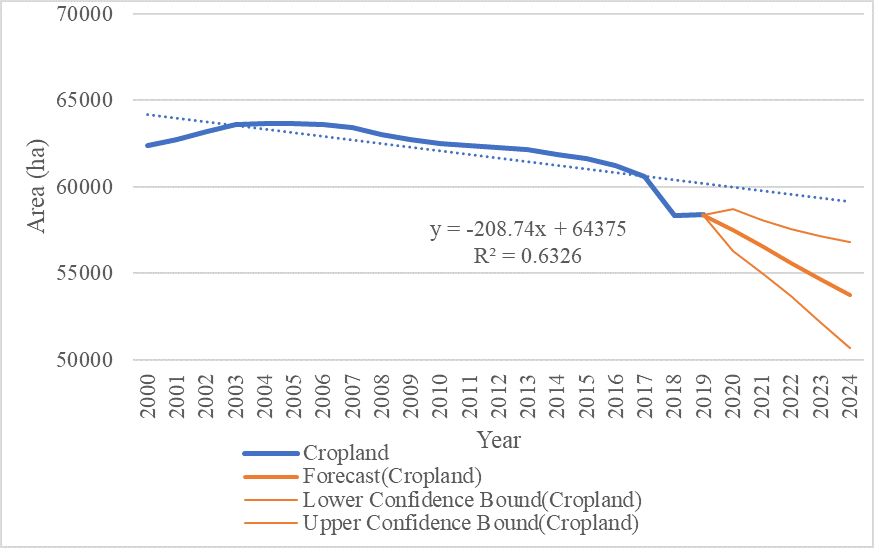
\includegraphics[width=0.8\textwidth]{images/banke_land_trend.png}
    \caption{Land Use Change Trend in Banke District (2000-2019)}
    \label{fig:Banke_land_trend}
\end{figure}

\begin{figure}[H]
    \centering
    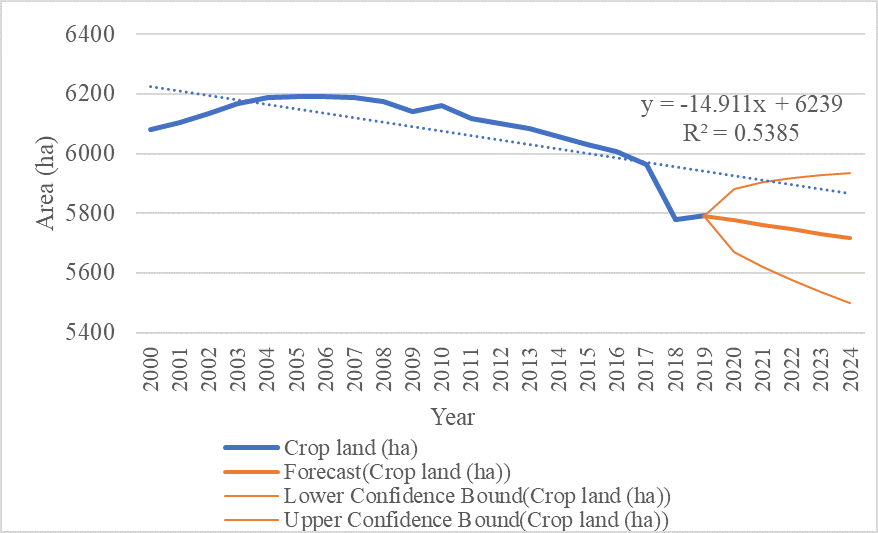
\includegraphics[width=0.8\textwidth]{images/janaki_land_trend.png}
    \caption{Land Use Change Trend in Janaki Rural Municipality (2000-2019)}
    \label{fig:Janaki_land_trend}
\end{figure}

\section{Discussion}
